% !TeX program = xelatex
\documentclass[UTF8,a4paper,11pt,fontset=none]{ctexart}
\usepackage[margin=22mm,top=21mm,bottom=23mm,headheight=16pt,headsep=9mm]{geometry}
\setCJKmainfont{Noto Serif CJK SC}
\setCJKsansfont{Noto Sans CJK SC}
\setmainfont{Liberation Serif}
\setsansfont{Liberation Sans}
\usepackage{amsmath,amssymb,mathtools,bm}
\usepackage{graphicx,tikz,tcolorbox,booktabs,tabularx,multirow,needspace}
\usepackage{enumitem,fancyhdr,lastpage,titlesec,xcolor,hyperref,array,multicol}
\usetikzlibrary{calc,arrows.meta,angles,quotes,3d}
\definecolor{navy}{HTML}{183F5D}
\definecolor{blue}{HTML}{276999}
\definecolor{light}{HTML}{EDF4F9}
\definecolor{teal}{HTML}{1A7668}
\definecolor{amber}{HTML}{986017}
\definecolor{warnbg}{HTML}{FFF5E9}
\definecolor{rulegray}{HTML}{DEE7ED}
\hypersetup{colorlinks=true,linkcolor=blue,urlcolor=blue,pdfauthor={Independent solution notes},pdftitle={空间解析几何第二章·习题2.1详解},pdfsubject={图形与方程、球面、坐标变换}}
\newcommand{\R}{\mathbb R}
\newcommand{\ans}[1]{\par\noindent\textcolor{teal}{\sffamily\bfseries 核查结论：}#1\par}
\newcommand{\idea}[1]{\par\noindent\textcolor{navy}{\sffamily\bfseries 思路：}#1\par}
\newcommand{\tip}[1]{\begin{tcolorbox}[colback=light,colframe=rulegray,boxrule=0.4pt,arc=1.5mm,left=3mm,right=3mm,top=2mm,bottom=2mm]#1\end{tcolorbox}}
\newcommand{\warning}[1]{\begin{tcolorbox}[colback=warnbg,colframe=amber,boxrule=0.55pt,arc=2mm,left=3mm,right=3mm,top=2mm,bottom=2mm]\textcolor{amber}{\sffamily\bfseries 提醒}\quad #1\end{tcolorbox}}
\newcommand{\Q}[2]{\par\Needspace{8\baselineskip}\phantomsection\addcontentsline{toc}{section}{第 #1 题：#2}\section*{第 #1 题\quad #2}\vspace{-1mm}}
\newcommand{\figcaptiontxt}[1]{\par\smallskip\noindent{\small\color{navy}\sffamily #1}\par}
\titleformat{\section}{\sffamily\Large\bfseries\color{navy}}{}{0pt}{}
\titlespacing*{\section}{0pt}{13pt}{8pt}
\setlength{\parindent}{2em}
\setlength{\parskip}{4pt}
\setlist[itemize]{leftmargin=2em,itemsep=2pt,topsep=4pt}
\setlist[enumerate]{leftmargin=2.2em,itemsep=2pt,topsep=4pt}
\allowdisplaybreaks[1]
\pagestyle{fancy}
\fancyhf{}
\fancyhead[L]{\textcolor{navy}{\footnotesize 空间解析几何 · 第二章详解}}
\fancyhead[R]{\textcolor{navy}{\footnotesize 第二章 / 习题 2.1}}
\fancyfoot[L]{\textcolor{gray}{\footnotesize v1.0 · 2026-10-16}}
\fancyfoot[R]{\textcolor{gray}{\footnotesize \thepage\,/\,\pageref{LastPage}}}
\renewcommand{\headrulewidth}{0.35pt}

\begin{document}
\thispagestyle{empty}
\vspace*{18mm}
{\sffamily\large\color{teal}\bfseries SPATIAL ANALYTIC GEOMETRY · VERIFIED NOTES}\par
\vspace{8mm}
{\sffamily\fontsize{28}{36}\selectfont\bfseries\color{navy} 第二章 空间解析几何}\par
\vspace{3mm}
{\sffamily\fontsize{20}{30}\selectfont\color{blue} 第一批：习题 2.1 \enspace 图形与方程}\par
\vspace{12mm}
\begin{tcolorbox}[colback=light,colframe=rulegray,arc=2mm,boxrule=0.6pt,left=5mm,right=5mm,top=5mm,bottom=5mm]
\large\textbf{本册范围}\par\medskip
\normalsize
本 PDF 先继续第二章的第一小节，覆盖\textbf{习题 2.1（题 1--7）}，重点是：
\begin{itemize}
\item 球面的建立与判定；
\item 曲线 / 曲面是否落在某个球面上；
\item 柱坐标、球坐标与直角坐标之间的转换；
\item 方程图像的几何意义判断。
\end{itemize}
题目来源为纸质页 51--52（PDF 页 57--58），书后答案页为纸质页 296--297（PDF 页 302--303）附近。
\end{tcolorbox}
\vfill
{\small\noindent\textbf{说明：}本稿延续第一章的做法：不用扫描页，改为可搜索文字重新整理；所有结论以独立推导为主，再与书后答案交叉核查。}\par
\clearpage
\begin{multicols}{2}
\footnotesize\setlength{\parskip}{0pt}\tableofcontents
\end{multicols}
\clearpage

\section*{本节知识框架与图形直观}
\addcontentsline{toc}{section}{本节知识框架与图形直观}
\tip{\textbf{主线一：球面。} 标准式
\[
(x-a)^2+(y-b)^2+(z-c)^2=R^2
\]
直接读出球心 $(a,b,c)$ 和半径 $R$。如果给的是一般二次式
\[
 x^2+y^2+z^2+2ax+2by+2cz+d=0,
\]
就先配方，再判断右边是否大于零。}

\begin{tcolorbox}[colback=white,colframe=rulegray,boxrule=0.4pt,arc=1.5mm,left=2mm,right=2mm,top=1.5mm,bottom=1.5mm]
\begin{minipage}[t]{0.49\linewidth}
\centering
\begin{tikzpicture}[scale=0.9,>=Stealth]
\draw[->] (-0.2,0)--(5.2,0) node[right]{$x$};
\draw[->] (0,-0.2)--(0,4.4) node[above]{$z$};
\draw[thick,blue] (2.3,2.0) circle (1.55);
\fill (2.3,2.0) circle(1.4pt) node[above right]{$C(a,c)$};
\draw[teal,->,thick] (2.3,2.0)--(3.75,2.0) node[midway,above]{$R$};
\fill (3.85,2.0) circle(1.2pt) node[right]{$P$};
\node at (2.55,0.55) {$CP=R$};
\node at (2.65,3.95) {球面标准式的截面直观};
\end{tikzpicture}
\figcaptiontxt{二维图里画成圆，空间里对应球面。配方的目的就是把方程化成“到定点距离等于常数”。}
\end{minipage}\hfill
\begin{minipage}[t]{0.47\linewidth}
\centering
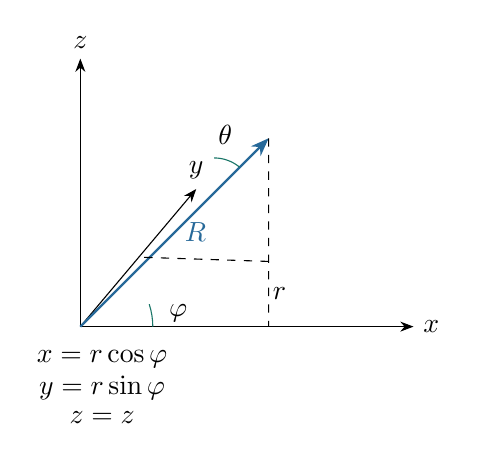
\begin{tikzpicture}[scale=0.92,>=Stealth]
\coordinate (O) at (0,0);
\draw[->] (O)--(4.6,0) node[right]{$x$};
\draw[->] (O)--(1.6,1.9) node[above]{$y$};
\draw[->] (O)--(0,3.7) node[above]{$z$};
\coordinate (P) at (2.6,2.6);
\draw[thick,blue,->] (O)--(P) node[midway,right]{$R$};
\coordinate (Q) at (2.6,0.9);
\draw[dashed] (P)--(Q)--(2.6,0);
\draw[dashed] (Q)--(0.77,0.96);
\draw[teal] (1.0,0) arc[start angle=0,end angle=18,radius=1.0];
\node at (1.35,0.18) {$\varphi$};
\draw[teal] (2.2,2.2) arc[start angle=50,end angle=90,radius=0.55];
\node at (2.0,2.65) {$\theta$};
\node at (2.75,0.45) {$r$};
\node at (0.3,-0.45) {$x=r\cos\varphi$};
\node at (0.3,-0.85) {$y=r\sin\varphi$};
\node at (0.3,-1.25) {$z=z$};
\end{tikzpicture}
\figcaptiontxt{柱坐标和球坐标的核心不是死记公式，而是先看：$r$ 是平面投影长度，$R$ 是空间距离，$\varphi$ 是方位角，$\theta$ 是与正 $z$ 轴的夹角。}
\end{minipage}
\end{tcolorbox}

\warning{题 6、题 7 很容易因为坐标记号混淆出错。本书球坐标采用 $(R,\varphi,\theta)$：其中 $\varphi$ 是平面方位角，$\theta$ 是与正 $z$ 轴的夹角，因此
\[
 x=R\sin\theta\cos\varphi,\quad y=R\sin\theta\sin\varphi,\quad z=R\cos\theta.
\]}

\Q{1}{写出球面的方程}
\idea{球面的本质是“到球心距离等于半径”。若已知直径端点，就先求中点当球心；若已知过一个圆，则圆所在平面上的圆心会落在球面与该平面的截圆中心上，再沿垂线补出球心。}

\textbf{(1) 以 $(1,0,2)$ 为球心，经过点 $(4,4,2)$。}
球心已知为 $C(1,0,2)$。半径由距离给出：
\[
R=\sqrt{(4-1)^2+(4-0)^2+(2-2)^2}=5.
\]
故球面方程为
\[
(x-1)^2+y^2+(z-2)^2=25.
\]

\textbf{(2) 以线段 $MN$ 为直径，$M(0,-2,4),N(2,-4,6)$。}
球心是直径中点：
\[
C=\left(1,-3,5\right).
\]
半径是 $MN$ 长度的一半：
\[
R=\frac12\sqrt{(2-0)^2+(-4+2)^2+(6-4)^2}=\sqrt{3}.
\]
故方程为
\[
(x-1)^2+(y+3)^2+(z-5)^2=3.
\]

\textbf{(3) 经过四点 $A(2,0,2),B(2,3,0),C(3,4,1),D(1,1,1)$。}
设球面为
\[
(x-u)^2+(y-v)^2+(z-w)^2=R^2.
\]
把四点代入，做“前式减后式”可消去 $R^2$，得到关于 $u,v,w$ 的线性方程组。解得
\[
u=\frac{11}{4},\qquad v=2,\qquad w=\frac74.
\]
再代回任一点（如 $A$）得
\[
R^2=\left(2-\frac{11}{4}\right)^2+(0-2)^2+\left(2-\frac74\right)^2=\frac{37}{8}.
\]
因此
\[
\left(x-\frac{11}{4}\right)^2+(y-2)^2+\left(z-\frac74\right)^2=\frac{37}{8}.
\]

\textbf{(4) 经过点 $(-1,-5,3)$，并经过圆}
\[
\begin{cases}
(x-1)^2+(y-1)^2+z^2=25,\\
z=0.
\end{cases}
\]
该圆位于平面 $z=0$ 上，圆心为 $(1,1,0)$，半径为 $5$。所有经过这个圆的球面，其球心都在过圆心且垂直于平面 $z=0$ 的直线上，故设球心为
\[
C=(1,1,k),\qquad R^2=25+k^2.
\]
代入点 $P(-1,-5,3)$：
\[
(-2)^2+(-6)^2+(3-k)^2=25+k^2.
\]
化简得 $k=4$，故
\[
R^2=25+16=41.
\]
所以球面方程为
\[
(x-1)^2+(y-1)^2+(z-4)^2=41.
\]

\textbf{(5) 经过点 $(-1,2,5)$，并且和三张坐标平面都相切。}
和三张坐标平面都相切，意味着球心到三个坐标平面的距离都等于半径 $R$，即球心坐标满足
\[
(|a|,|b|,|c|)=(R,R,R).
\]
因此球心只能在八个点 $(\pm R,\pm R,\pm R)$ 中选。又因为给定点 $(-1,2,5)$ 的符号特征最接近 $(-,+,+)$，设球心为 $(-R,R,R)$。代入过点条件：
\[
(-1+R)^2+(2-R)^2+(5-R)^2=R^2.
\]
化简得
\[
R^2-8R+15=0\quad\Longrightarrow\quad R=3\ \text{或}\ 5.
\]
于是得到两个球面：
\[
(x+3)^2+(y-3)^2+(z-3)^2=9,
\]
\[
(x+5)^2+(y-5)^2+(z-5)^2=25.
\]
\ans{与书后答案一致：5 个小问分别对应书后列出的 5 个结果。}

\Q{2}{判别给定二次方程是否表示球面}
\idea{凡是形如 $x^2+y^2+z^2+2ax+2by+2cz+d=0$ 的式子，都先配成
\[
(x+a)^2+(y+b)^2+(z+c)^2=a^2+b^2+c^2-d.
\]
右边大于 $0$ 才是球面；等于 $0$ 是一个点；小于 $0$ 则无实点。}

\begin{enumerate}[label=(\arabic*)]
\item $x^2+y^2+z^2+2x-4y+4z=0$

配方：
\[
(x+1)^2+(y-2)^2+(z+2)^2=9.
\]
所以是球面，球心 $(-1,2,-2)$，半径 $3$。

\item $x^2+y^2+z^2-8x-2y+4z-4=0$

配方：
\[
(x-4)^2+(y-1)^2+(z+2)^2=25.
\]
所以是球面，球心 $(4,1,-2)$，半径 $5$。

\item $x^2+y^2+z^2+2x-4y+6z+15=0$

配方后得
\[
(x+1)^2+(y-2)^2+(z+3)^2= -1.
\]
右边为负，所以无实点，不是球面。

\item $x^2+y^2+z^2+4x+2y+12z+41=0$

配方后得
\[
(x+2)^2+(y+1)^2+(z+6)^2=0.
\]
所以图像退化为一点 $(-2,-1,-6)$，不是球面。
\end{enumerate}
\ans{与书后答案一致：前两问是球面，后两问分别是空集与一点。}

\Q{3}{什么时候表示球面？}
题目给出
\[
x^2+y^2+z^2+2ax+2by+2cz+d=0.
\]
配方得
\[
(x+a)^2+(y+b)^2+(z+c)^2=a^2+b^2+c^2-d.
\]
若要图像是一个真正的球面，那么右边必须严格大于零，所以充分必要条件是
\[
a^2+b^2+c^2>d.
\]
若恰好等于 $d$，图像退化成一点；若小于 $d$，则无实图像。
\ans{结论：$a^2+b^2+c^2>d$。与书后答案一致。}

\Q{4}{说明下列曲线都在一个球面上}
\idea{所谓“在一个球面上”，就是能从已知关系推出某个固定的球面方程。一般通过直接计算 $x^2+y^2+z^2$，或者把式子整理成配方形式。}

\textbf{(1)} 若
\[
\begin{cases}
 x=3\sin\phi,\\
 y=4\sin\phi,\\
 z=5\cos\phi,
\end{cases}
\]
则
\[
 x^2+y^2+z^2=9\sin^2\phi+16\sin^2\phi+25\cos^2\phi=25.
\]
故曲线在球面
\[
 x^2+y^2+z^2=25
\]
上。

\textbf{(2)} 若
\[
 x=\frac{t}{1+t^2+t^4},\qquad y=\frac{t^2}{1+t^2+t^4},\qquad z=\frac{t^3}{1+t^2+t^4},
\]
则
\[
 x^2+y^2+z^2=\frac{t^2+t^4+t^6}{(1+t^2+t^4)^2}=\frac{t^2(1+t^2+t^4)}{(1+t^2+t^4)^2}=\frac{t^2}{1+t^2+t^4}=y.
\]
所以
\[
 x^2+y^2+z^2=y
\]
即
\[
 x^2+\left(y-\frac12\right)^2+z^2=\frac14.
\]
这是一张球面。

\textbf{(3)} 若
\[
\begin{cases}
 x^2+3y^2+5z^2=5,\\
 2y^2+4z^2=3,
\end{cases}
\]
两式相减得
\[
 x^2+y^2+z^2=2.
\]
故该曲线落在球面
\[
 x^2+y^2+z^2=2
\]
上。
\ans{三问都可以独立推出一个固定球面方程，因此都在某个球面上。}

\Q{5}{求方程（组）的图像}
\textbf{(1)}
\[
(x^2+y^2+z^2-4)(x^2+y^2+z^2-9)=0.
\]
积为零，说明至少有一个因子为零，所以图像是两张同心球面：
\[
 x^2+y^2+z^2=4 \quad\text{或}\quad x^2+y^2+z^2=9.
\]
也就是以原点为球心、半径分别为 $2$ 和 $3$ 的两张球面。

\textbf{(2)}
\[
(x^2+y^2+z^2-25)^2+\Big((x-2)^2+(y+1)^2+(z-2)^2-16\Big)^2=0.
\]
两个平方和等于零，只能两项都为零，因此图像是方程组
\[
\begin{cases}
 x^2+y^2+z^2=25,\\
 (x-2)^2+(y+1)^2+(z-2)^2=16
\end{cases}
\]
的公共部分，即两张球面的交线。
第一张球面球心 $O(0,0,0)$，半径 $5$；第二张球面球心 $C(2,-1,2)$，半径 $4$。两球心距
\[
OC=\sqrt{2^2+(-1)^2+2^2}=3.
\]
满足
\[
|5-4|<3<5+4,
\]
故两球面相交于一个圆。因此图像是一条圆周。
\ans{(1) 两张同心球面；(2) 两球面的交圆。}

\Q{6}{坐标系之间的转换}
\idea{本题一律遵循：
\[
 x=r\cos\varphi,\ y=r\sin\varphi,\ z=z;
\qquad
 x=R\sin\theta\cos\varphi,\ y=R\sin\theta\sin\varphi,\ z=R\cos\theta.
\]
转换时最好先画出投影长度：$r=\sqrt{x^2+y^2}$，$R=\sqrt{x^2+y^2+z^2}$。}

\textbf{(1) 由直角坐标求柱坐标和球坐标}
\begin{enumerate}[label=\textcircled{\arabic*}]
\item $(1,1,1)$：
\[
 r=\sqrt{1^2+1^2}=\sqrt2,\quad \varphi=\frac\pi4,\quad z=1.
\]
故柱坐标为 $\bigl(\sqrt2,\frac\pi4,1\bigr)$。
又
\[
 R=\sqrt{1+1+1}=\sqrt3,\qquad \theta=\arccos\frac{1}{\sqrt3}.
\]
故球坐标为
\[
\left(\sqrt3,\frac\pi4,\arccos\frac{1}{\sqrt3}\right).
\]

\item $(0,-2,1)$：
\[
 r=2,\quad \varphi=\frac{3\pi}{2},\quad z=1;
\]
故柱坐标为 $\left(2,\frac{3\pi}{2},1\right)$。
再算
\[
 R=\sqrt5,\qquad \theta=\arccos\frac{1}{\sqrt5}.
\]
故球坐标为
\[
\left(\sqrt5,\frac{3\pi}{2},\arccos\frac{1}{\sqrt5}\right).
\]

\item $(0,0,1)$：
柱坐标里 $r=0$，故方位角 $\varphi$ 不唯一：
\[
(0,\varphi,1),\quad \varphi\in[0,2\pi).
\]
球坐标里 $R=1,\theta=0$，此时 $\varphi$ 同样任意：
\[
(1,\varphi,0),\quad \varphi\in[0,2\pi).
\]
\end{enumerate}

\textbf{(2) 由球坐标求直角坐标和柱坐标}
\begin{enumerate}[label=\textcircled{\arabic*}]
\item $\left(1,\frac{4\pi}{3},\frac\pi4\right)$：
\[
 x=\sin\frac\pi4\cos\frac{4\pi}{3}=-\frac{\sqrt2}{4},\quad
 y=\sin\frac\pi4\sin\frac{4\pi}{3}=-\frac{\sqrt6}{4},\quad
 z=\cos\frac\pi4=\frac{\sqrt2}{2}.
\]
柱坐标中
\[
 r=R\sin\theta=\frac{\sqrt2}{2},
\]
所以柱坐标为
\[
\left(\frac{\sqrt2}{2},\frac{4\pi}{3},\frac{\sqrt2}{2}\right).
\]

\item $\left(2,\frac{3\pi}{4},\frac\pi3\right)$：
\[
 x=2\cdot \frac{\sqrt3}{2}\cdot\left(-\frac{\sqrt2}{2}\right)=-\frac{\sqrt6}{2},\quad
 y=2\cdot \frac{\sqrt3}{2}\cdot\frac{\sqrt2}{2}=\frac{\sqrt6}{2},\quad z=2\cdot\frac12=1.
\]
柱坐标为
\[
\left(\sqrt3,\frac{3\pi}{4},1\right).
\]

\item $(a,120^\circ,135^\circ)$：
\[
 x=a\sin135^\circ\cos120^\circ=-\frac{\sqrt2}{4}a,
\]
\[
 y=a\sin135^\circ\sin120^\circ=\frac{\sqrt6}{4}a,
\]
\[
 z=a\cos135^\circ=-\frac{\sqrt2}{2}a.
\]
柱坐标为
\[
\left(\frac{\sqrt2}{2}a,120^\circ,-\frac{\sqrt2}{2}a\right).
\]
\end{enumerate}

\textbf{(3) 由柱坐标求直角坐标和球坐标}
\begin{enumerate}[label=\textcircled{\arabic*}]
\item $(2,60^\circ,-2)$：
\[
 x=2\cos60^\circ=1,\qquad y=2\sin60^\circ=\sqrt3,\qquad z=-2.
\]
再求
\[
 R=\sqrt{1+3+4}=2\sqrt2,
\]
且
\[
 \varphi=60^\circ,\qquad \theta=\arccos\frac{-2}{2\sqrt2}=135^\circ.
\]
故球坐标为
\[
(2\sqrt2,60^\circ,135^\circ).
\]

\item $(2,225^\circ,5)$：
\[
 x=2\cos225^\circ=-\sqrt2,
\quad y=2\sin225^\circ=-\sqrt2,
\quad z=5.
\]
再求
\[
 R=\sqrt{2+2+25}=\sqrt{29},\qquad \theta=\arccos\frac{5}{\sqrt{29}}.
\]
故球坐标为
\[
\left(\sqrt{29},225^\circ,\arccos\frac{5}{\sqrt{29}}\right).
\]
\end{enumerate}
\ans{与书后答案页列出的结果一致；第 3 个点和第 3 个球坐标都要注意“角可以不唯一”的情况。}

\Q{7}{把柱坐标 / 球坐标方程化成直角坐标方程并解释几何意义}
\textbf{(1) }$r=1$。
由 $r^2=x^2+y^2$ 得
\[
 x^2+y^2=1.
\]
因为与 $z$ 无关，所以图像是以 $z$ 轴为轴、半径为 $1$ 的圆柱面。

\textbf{(2) }$2\le R\le 4$。
由 $R^2=x^2+y^2+z^2$ 得
\[
 4\le x^2+y^2+z^2\le 16.
\]
这是两张同心球面之间（包含边界）的部分，即球壳。

\textbf{(3) }$r=2\sin\varphi\;(0\le \varphi\le \pi)$。
两边乘以 $r$：
\[
 r^2=2r\sin\varphi.
\]
利用 $r^2=x^2+y^2$，$r\sin\varphi=y$，得
\[
 x^2+y^2=2y.
\]
整理为
\[
 x^2+(y-1)^2=1.
\]
同样与 $z$ 无关，所以是圆柱面，其母圆在 $xOy$ 平面上是圆心 $(0,1)$、半径 $1$ 的圆。

\textbf{(4) }$R=4\cos\theta\;(0\le \theta\le \pi/2)$。
由 $z=R\cos\theta$ 可知
\[
 R^2=4z.
\]
再代入 $R^2=x^2+y^2+z^2$，得到
\[
 x^2+y^2+z^2=4z.
\]
配方得
\[
 x^2+y^2+(z-2)^2=4.
\]
因此图像是球心 $(0,0,2)$、半径 $2$ 的球面。由于该球面本身就在 $z\ge 0$ 范围内，所以角条件并没有再额外删去点。
\ans{四个图像分别是：圆柱面、球壳、圆柱面、球面。与书后答案一致。}

\clearpage
\section*{本批复习小结}
\addcontentsline{toc}{section}{本批复习小结}
\begin{enumerate}
\item \textbf{球面题的万能入口：}先找球心，再找半径；如果是一般式，就配方。
\item \textbf{判断是不是球面：}右边常数 $>0$ 才是球面；$=0$ 是一点；$<0$ 是空集。
\item \textbf{坐标变换不要死背：}先理解 $r,R,\varphi,\theta$ 的几何意义，再写公式。
\item \textbf{方程图像判断：}看到“只含 $x,y$ 不含 $z$”，通常就是沿 $z$ 方向拉伸出来的柱面；看到“只含 $x^2+y^2+z^2$”，优先想到球面对称性。
\end{enumerate}
\tip{\textbf{接下来可继续做的内容：}第二章下一批最自然就是 \textbf{习题 2.2（平面的方程）} 和 \textbf{习题 2.3（直线的方程）}。这两部分和考研里“平面 / 直线方程、位置关系”的基础训练联系最紧。}

\end{document}
